\begin{previewactivity}[\textbf{Constructing a New Function}] \label{PA:compositionintro} \hfill \\
Let  $A = \left\{ {a, b, c, d} \right\}$, $B = \left\{ {p, q, r} \right\}$, and  
$C = \left\{ {s, t, u, v} \right\}$.  The arrow diagram in Figure~\ref{fig:preview64} shows two functions:  
$f\x A \to B$  and  $g\x B \to C$.
\begin{figure}[h]
\begin{center}
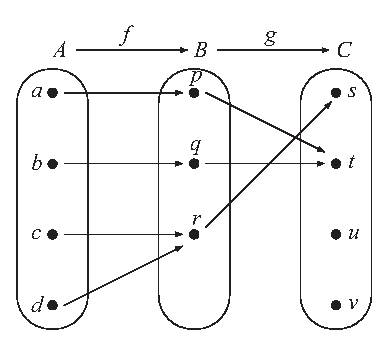
\includegraphics{figps-prev641.eps} 
\caption{Arrow Diagram Showing Two Functions} \label{fig:preview64}
\end{center}
\end{figure}
Notice that if $x \in A$, then $f(x) \in B$.  Since $f(x) \in B$, we can apply the function $g$ to $f(x)$, and we obtain 
$g(f(x))$, which is an element of $C$.

%Notice that $a \in A$ and $ f(a) = p$.  Since $p \in B$, we can use the function $g$ and obtain 
%$g(p) = t$.  This can be summarized as follows:
%\[
%g ( f(a) ) = g(p) = t.
%\]
Using this process, determine $g(f(a))$, $g ( f(b) )$, $g ( f(c) )$, and 
$g ( f(d) )$.  Then explain how we can use this information to define a function from $A$ to $C$.

%Complete the following table.  For example,  if  $x = a$, then  $f( a ) = p$, and  $g( {f( a )} ) = g( p ) = t$.
%\begin{center}
%\begin{tabular}{ c  | c | c}
% $x$  &  $f( x )$  &  $g( {f( x )} )$ \\ \hline
% $a$  &                       &                                        \\ \hline
% $b$  &                       &                                        \\ \hline
% $c$  &                       &                                        \\ \hline
% $d$  &                       &                                        \\ \hline
%\end{tabular}
%\end{center}
%Explain how this table defines a function from  $A$  to  $C$.
\end{previewactivity}
%\hbreak

\endinput
